\cleardoublepage

\chapter{Large Language Models (LLMs)}
\label{Large Language Models (LLMs)}

\section{Introducción}
Los Modelos de Lenguaje de Gran Escala (LLMs) han demostrado capacidades notables en tareas de procesamiento de lenguaje natural y más allá. Estos modelos han revolucionado el campo del NLP y se han postulado como los modelos a resolver el problema de la generación de texto. 
Para este capítulo se ha usado la revisión \textit{A Comprehensive Overview of Large Language Models} \citep{naveed2023comprehensive}

\section{Generación de Texto}
La generación de texto es una de las tareas fundamentales que los LLMs intentan resolver. Este problema consiste en producir secuencias de texto coherente y relevante a partir de una entrada dada. La tarea puede implicar varios subproblemas, como la continuación de un texto, la respuesta a preguntas, la traducción automática, entre otros.

El enfoque principal para resolver la generación de texto en LLMs es la predicción del siguiente token. Esto implica modelar la probabilidad condicional de cada token dado el contexto de los tokens anteriores. Formalmente, si tenemos una secuencia de tokens \( t_1, t_2, ..., t_n \), el modelo aprende a predecir la probabilidad del token \( t_{n+1} \) basándose en los tokens \( t_1, t_2, ..., t_n \). Este proceso se puede expresar como:
\[ P(t_{n+1} | t_1, t_2, ..., t_n) \]
Para entrenar este tipo de modelos, se utilizan corpus grandes de texto en el cual el modelo ajusta sus parámetros para maximizar la probabilidad de los tokens siguientes.

\section{Historia y Evolución de los LLMs}
La evolución de los modelos de lenguaje natural ha sido marcada por avances significativos en las técnicas y arquitecturas utilizadas. Desde los primeros modelos estadísticos hasta los avanzados modelos de lenguaje de gran escala (LLMs), el campo ha experimentado una transformación profunda.

\subsection{Modelos de Lenguaje Estadísticos}
Los primeros enfoques para el procesamiento de lenguaje natural se basaban en modelos estadísticos. Estos modelos utilizaban probabilidades para predecir la aparición de palabras en un contexto dado. Un ejemplo típico es el modelo de n-gramas, que calcula la probabilidad de una palabra basándose en las n-1 palabras anteriores. Aunque efectivos en ciertos contextos, estos modelos tenían limitaciones significativas en su capacidad para capturar dependencias a largo plazo y gestionar vocabularios extensos.

\subsection{Modelos de Lenguaje Neurales}
Con el advenimiento de las redes neuronales, los modelos de lenguaje experimentaron un cambio paradigmático. Los modelos de lenguaje neurales, como los basados en redes neuronales recurrentes (RNNs), ofrecieron mejoras en la capacidad de modelado y generalización. Sin embargo, a pesar de estas mejoras, las RNNs enfrentaban desafíos en la captura de dependencias a largo plazo debido al problema del gradiente desvaneciente. Las arquitecturas como LSTM (Long Short-Term Memory) y GRU (Gated Recurrent Unit) fueron desarrolladas para mitigar estos problemas.

\subsection{Transformers y su Impacto}
El verdadero avance en los modelos de lenguaje vino con la introducción de los Transformers, presentados por Vaswani et al. en 2017 \citep{vaswani2017attention}. Los Transformers se basan en un mecanismo de autoatención que permite al modelo considerar todas las posiciones en la secuencia de entrada simultáneamente, superando las limitaciones de las RNNs en cuanto a la captura de dependencias a largo plazo. Esta arquitectura revolucionó el campo y llevó al desarrollo de modelos preentrenados como BERT (Bidirectional Encoder Representations from Transformers) y GPT (Generative Pre-trained Transformer). La Figura \ref{fig:transformer_architecture} muestra la arquitectura básica de un Transformer.

\begin{figure}[h]
\centering
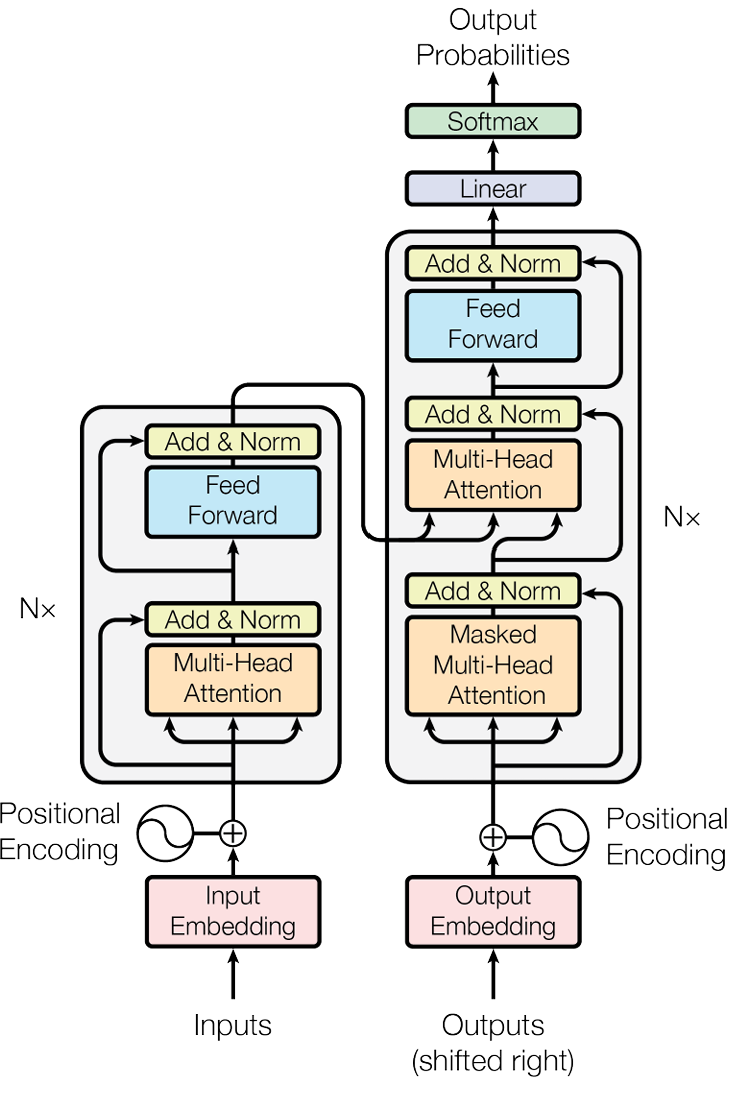
\includegraphics[width=0.3\textwidth]{figuras/capitulo1/transformer_architecture.png}
\caption{Arquitectura básica de un Transformer.}
\label{fig:transformer_architecture}
\end{figure}

\subsection{Transición de PLMs a LLMs}
La transición de los modelos de lenguaje preentrenados (PLMs) a los modelos grandes del lenguaje (LLMs) se caracterizó por un aumento significativo en el tamaño de los modelos y la cantidad de datos de entrenamiento. Modelos como GPT-3, con 175 mil millones de parámetros, demostraron que el escalado de los modelos y los datos de entrenamiento puede llevar a mejoras drásticas en el rendimiento en una amplia gama de tareas de NLP. Los LLMs han mostrado capacidades sorprendentes en tareas de zero-shot y few-shot learning, donde pueden realizar tareas no vistas durante el entrenamiento con poca o ninguna adaptación adicional. La Figura \ref{fig:llm_evolution} muestra la evolución cronológica de los principales LLMs.

\begin{figure}[h]
\centering
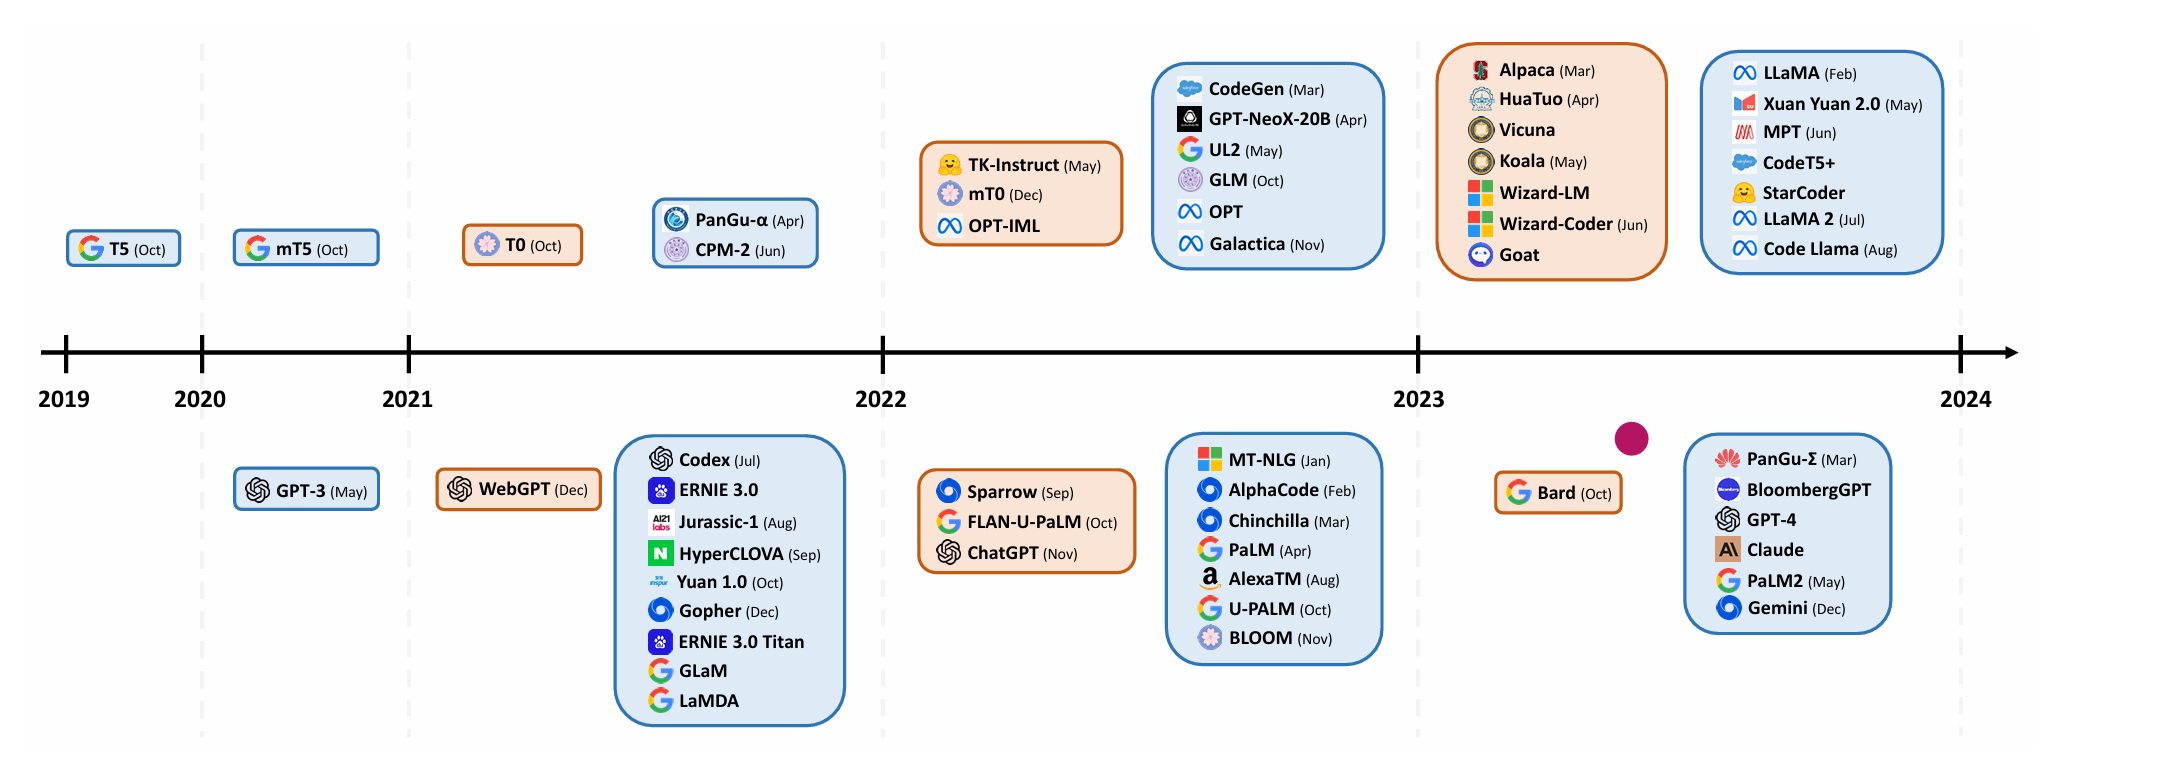
\includegraphics[width=0.85\textwidth]{figuras/capitulo1/llm_evolution.png}
\caption{Evolución cronológica de los principales LLMs.}
\label{fig:llm_evolution}
\end{figure}


\section{Arquitecturas y Modelos Importantes}
En los últimos años, los Modelos grandes del lenguaje (LLMs) han experimentado avances significativos, lo que ha resultado en la creación de arquitecturas y modelos innovadores. Estos modelos no solo han mejorado en términos de capacidad y precisión, sino que también han introducido nuevas formas de abordar problemas complejos en el procesamiento de lenguaje natural. A continuación, se presentan algunas de las arquitecturas históricas y modelos más importantes en el ámbito de los LLMs.

\subsection{T5 (Text-to-Text Transfer Transformer)}
El modelo T5, desarrollado por Google, es un modelo de codificador-decodificador que trata todas las tareas de procesamiento de lenguaje natural (NLP) como problemas de generación de texto. Esto significa que convierte todas las tareas de entrada en una estructura de texto a texto, lo que permite un enfoque unificado para diversas tareas de NLP.

\begin{figure}[h]
\centering
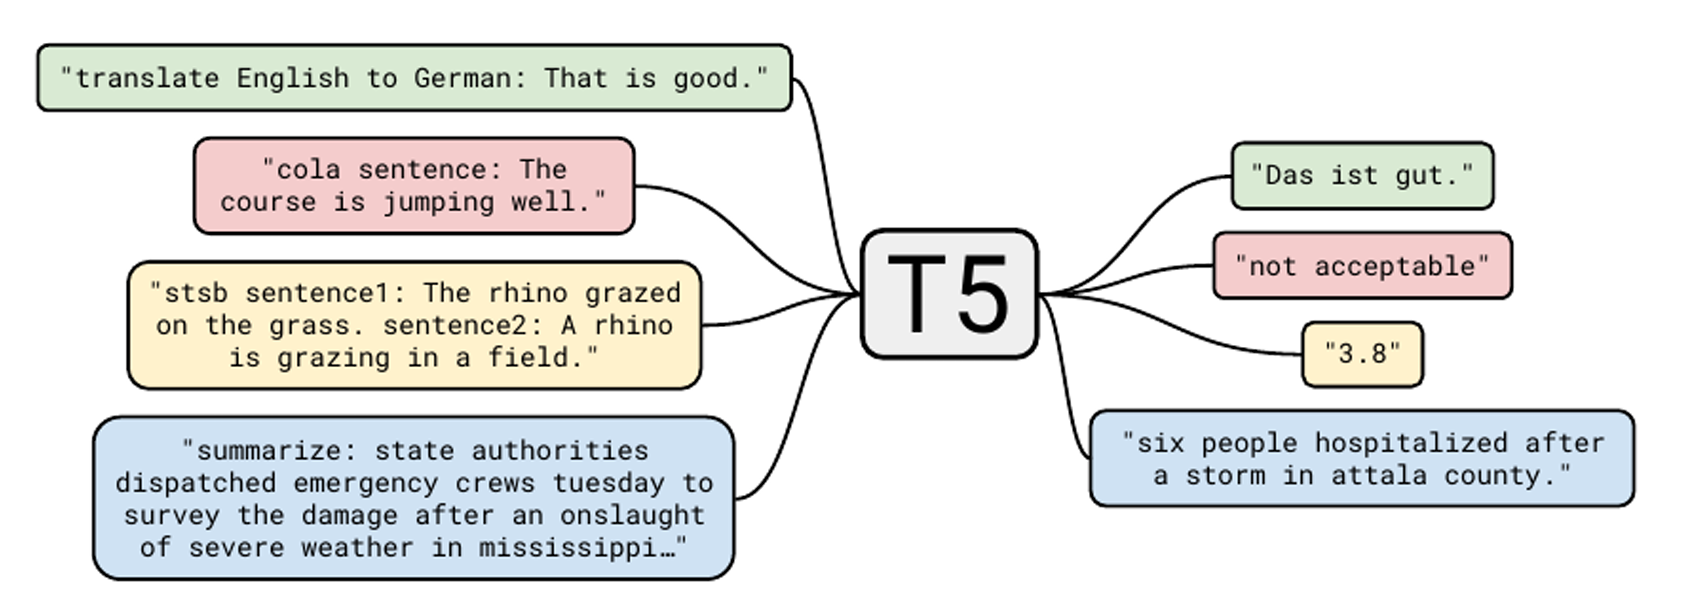
\includegraphics[width=0.85\textwidth]{figuras/capitulo1/t5.png}
\caption{Ejemplo unificado de formación texto a texto, imagen origen de \citep{raffel2020exploring}}
\label{fig:llm_evolution}
\end{figure}

\subsection{BERT (Bidirectional Encoder Representations from Transformers)}
BERT, desarrollado por Google \citep{devlin2018bert}, es un modelo basado en transformers que se entrena utilizando un objetivo de modelado de lenguaje enmascarado, donde se predicen tokens enmascarados dentro de una secuencia utilizando el contexto bidireccional de la secuencia completa. Este enfoque permite a BERT capturar relaciones más complejas y contextuales en el texto en comparación con los modelos unidireccionales. La capacidad de BERT para ser finetuneado de manera eficiente sin requerir modificaciones sustanciales en la arquitectura específica de cada tarea ha contribuido significativamente a su adopción y éxito en múltiples dominios de NLP.

\subsection{mT5 (Multilingual T5)}
mT5 es una variante multilingüe del modelo T5, entrenada en el dataset mC4 que abarca 101 idiomas. Este modelo utiliza un vocabulario más amplio de 250,000 tokens para cubrir múltiples lenguajes. Para evitar el sobreajuste o subajuste en un idioma específico, mT5 emplea un procedimiento de muestreo de datos que selecciona muestras de todos los idiomas. Además, durante el afinamiento para tareas específicas utilizando datos en inglés, el modelo puede generar salidas correctas en otros idiomas.

\subsection{GPT-3 (Generative Pre-trained Transformer 3)}
GPT-3, desarrollado por OpenAI, es uno de los modelos de lenguaje más grandes y avanzados hasta la fecha, con 175 mil millones de parámetros. GPT-3 utiliza una arquitectura de transformers similar a GPT-2 pero con atención densa y dispersa en las capas del transformer. Este modelo demostró que el escalado masivo del tamaño del modelo y los datos de entrenamiento puede llevar a mejoras significativas en el rendimiento en una amplia gama de tareas de NLP. GPT-3 es especialmente conocido por su capacidad de realizar tareas en configuraciones de zero-shot, few-shot y one-shot learning, proporcionando respuestas coherentes y contextualmente relevantes. \hfill \break

\begin{figure}[h]
\centering
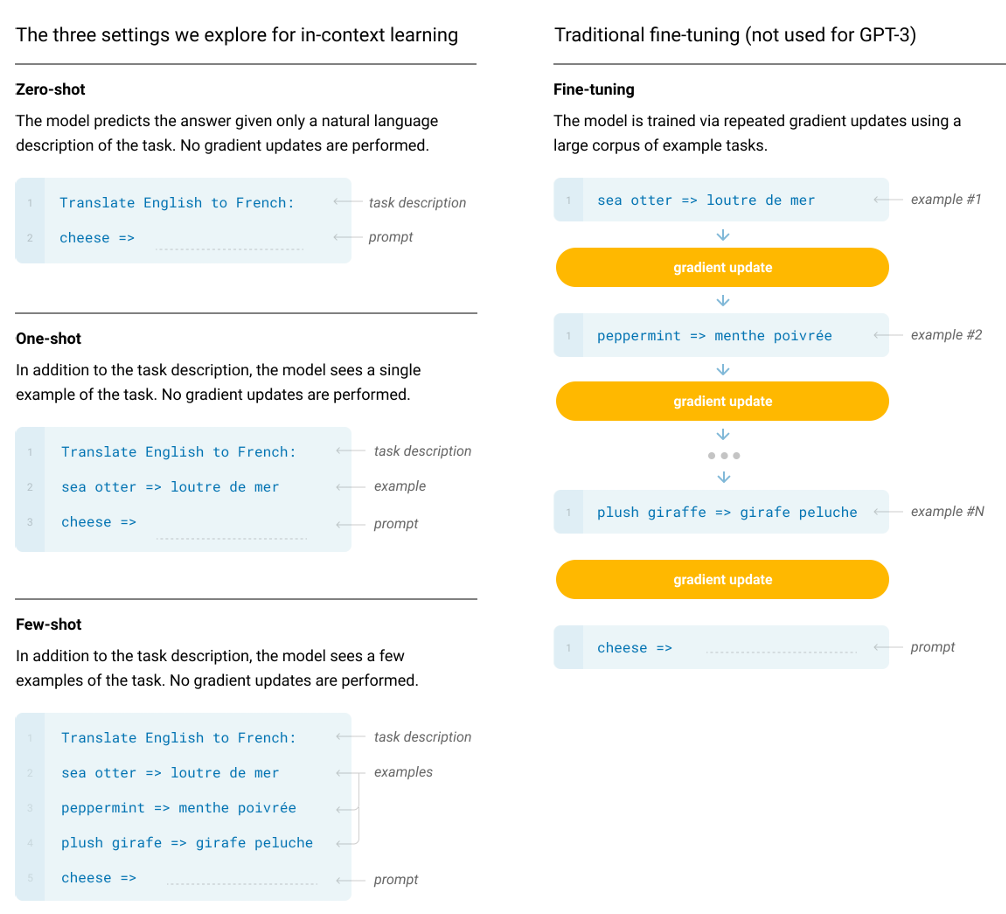
\includegraphics[width=0.6\textwidth]{figuras/capitulo1/gpt3.png}
\caption{Zero-shot, one-shot y few-shot contrastado con finetunning tradicional. Imagen origen de \citep{brown2020language}}
\label{fig:llm_evolution}
\end{figure}


Entre todos estos avances han llegado infinidad de modelos y arquitecturas que han presentado avances significativos en el ámbito del NLP creando un antes y un después en la figura de los LLMs, véase en la figura \ref{fig:llm_evolution}. Desde modelos abiertos como Llama (meta) y Mistral hasta modelos propietarios como GPT4 (OpenAI) o Claude (Anthropic) en sus diferentes versiones.


\section{Aplicaciones de los LLMs}
\subsection{Generación de Texto}

\subsection{Resumen Automático}

\subsection{Traducción Automática}

\subsection{Interacción Conversacional}

\subsection{Respuesta a Preguntas}


\section{Desafíos y Futuras Direcciones}
\subsection{Costos Computacionales y Energéticos}

\subsection{Generalización y Adaptación de Dominios}

\subsection{Seguridad y Ética}

\subsection{Privacidad y Datos Sensibles}

